\chapter{Introducción}
\label{cap:capitulo1}
\setcounter{page}{1}

\begin{flushright}
\begin{minipage}[]{10cm}
\emph{La automatización no es el enemigo del trabajador, sino la clave para su evolución}\\
\end{minipage}\\
\end{flushright}

\vspace{1cm}

La automatización ha sido un pilar fundamental en el desarrollo de la industria moderna, permitiendo mejoras significativas en eficiencia, calidad y seguridad. Desde la Revolución Industrial hasta la actualidad, la evolución de las tecnologías ha dado paso a sistemas cada vez más sofisticados, donde la integración de robots ha transformado los entornos de producción, ofreciendo resultados de mayor calidad y reduciendo costes y tiempos de producción. En particular, la robótica industrial ha desempeñado un papel clave en sectores como la automoción, la electrónica y la manufactura, ofreciendo soluciones flexibles y altamente eficientes para la producción en serie.\\

En este capítulo se presentará el contexto en el que se desarrolla este trabajo, proporcionando una visión general de la automatización en la industria y su evolución hasta la actualidad. Posteriormente, se acotará el enfoque hacia la robótica industrial, destacando su impacto en la optimización de procesos productivos. Finalmente, se delimitará el ámbito específico de este estudio, centrado en la automatización de una línea de producción robotizada, analizando sus beneficios, retos y las tecnologías empleadas.

\section{La robótica}
\label{sec:miseccion} % etiqueta para luego referenciar esta sección

La robótica es la disciplina científica que integra conocimientos de electrónica, mecánica e informática para desarrollar sistemas automatizados capaces de realizar tareas de manera autónoma o semiautónoma. Los componentes que conforman un robot son esenciales para su funcionamiento, desde la estructura mecánica (brazos, ruedas, actuadores, etc.), que debe garantizar un movimiento preciso y estabilidad, hasta los sistemas electrónicos que deben ser totalmente compatibles y funcionales para permitir la correcta operación. Además, los algoritmos que se implementan deben ser robustos, seguros y capaces de adaptarse a diversas situaciones y condiciones del entorno. \\

En el ámbito de la robótica, los sensores juegan un papel crucial, ya que proporcionan al robot la información necesaria sobre su entorno. Estos sensores, de diversos tipos, miden una amplia gama de magnitudes físicas, como la luz, posición, velocidad, fuerza, temperatura..., funcionando de manera análoga a los órganos sensoriales en los seres humanos. \\

Una vez que los sensores recogen los datos del entorno, el software del robot procesa esta información, proporcionando la inteligencia necesaria para tomar decisiones. Utilizando algoritmos avanzados o inteligencia artificial, el robot es capaz de generar respuestas adecuadas a las entradas, lo que resulta en la ejecución de una acción específica, como un movimiento o la interacción con su entorno. \\

Finalmente, los actuadores son los encargados de ejecutar las acciones determinadas por el sistema de control, permitiendo que el robot lleve a cabo tareas como moverse o manipular objetos. Los actuadores son fundamentales para la efectividad del robot, ya que son los elementos que materializan las decisiones procesadas en acciones físicas tangibles. 

\begin{figure} [h!]
  \begin{center}
    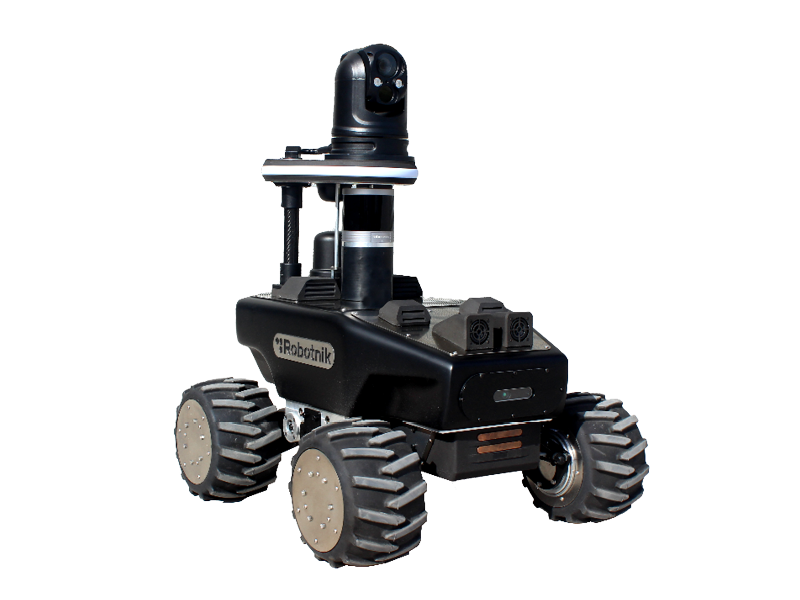
\includegraphics[width=11cm]{figs/Robot_intro}
  \end{center}
  \caption{\centering RB-WATCHER de Robotink.}
  \label{fig:Robot_intro}
\end{figure}

\subsection{Robótica de Servicio}
\label{sec:subseccion_1}

La robótica de servicio engloba los robots diseñados para interactuar con personas o realizar tareas útiles en un entorno no industrial. Estos robots se emplean para proporcionar servicios en lugar de realizar trabajos repetitivos de manufactura, y están diseñados para facilitar tareas cotidianas, mejorar la calidad de vida o asistir a los seres humanos en áreas específicas. \\

La robótica de servicio abarca una amplia gama de aplicaciones en sectores tan diversos como la agricultura, minería, rescate, logística y conducción autónoma. Estos robots suelen ser principalmente móviles, ya que requieren desplazarse por su entorno para realizar sus tareas. Además, deben ser reactivos a las condiciones del medio y lo suficientemente robustos para garantizar el éxito de su misión, incluso en entornos impredecibles. Generalmente, estos robots tienen menos de tres grados de libertad debido a la naturaleza de las tareas que realizan, las cuales no requieren movimientos extremadamente complejos. Actúan en entornos no controlados, lo que implica que su programación y control deben ser altamente adaptativos, provocando que la programación sea especialmente compleja en ciertos escenarios \footnote{Deiscar, B. ¿Qué es la robótica de servicio? UDIT Universidad; UDIT - Universidad de Diseño y Tecnología. \url{https://udit.es/actualidad/que-es-la-robotica-de-servicio/}}. 

\begin{figure} [h!]
  \begin{center}
    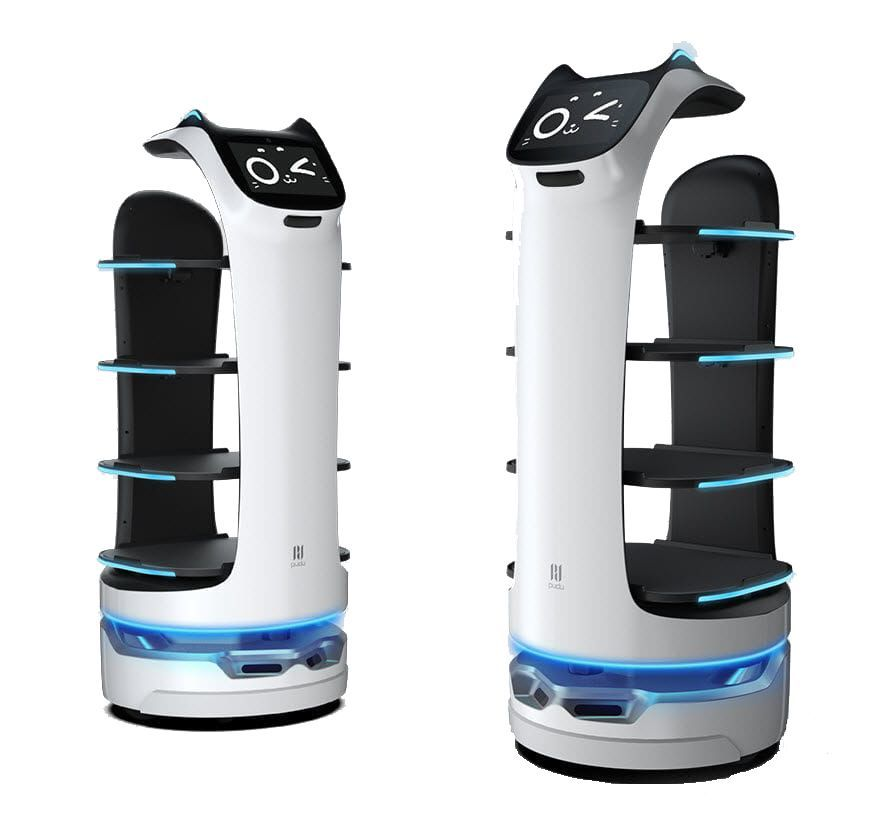
\includegraphics[width=8cm]{figs/robotica_servicio}
  \end{center}
  \caption{\centering Pudu bellabot.}
  \label{fig:robotica_servicio}
\end{figure}

\subsection{Robótica Industrial}

La robótica industrial es una disciplina de la ingeniería robótica dedicada al diseño, desarrollo y fabricación de robots industriales con el propósito de automatizar tareas repetitivas tradicionalmente realizadas por seres humanos. Estos sistemas robóticos se caracterizan por seguir una secuencia de instrucciones predefinidas, ejecutando ciclos de trabajo continuos en líneas de producción de diversos sectores industriales. Su uso es particularmente frecuente en la industria manufacturera, donde contribuyen significativamente a mejorar la eficiencia, la velocidad y la calidad de los procesos productivos \footnote{(N.d.). Unir.net. Retrieved February 24, 2025, from \url{https://www.unir.net/revista/ingenieria/robotica-industrial/}}. 

A diferencia de los robots de servicio, los robots industriales operan en entornos altamente controlados, lo que simplifica su programación y control. Debido a estas condiciones estables, estos robots suelen tener más de tres grados de libertad, permitiéndoles realizar movimientos complejos con gran precisión. Aunque su aplicación principal ha sido históricamente en entornos industriales, su uso se ha expandido hacia sectores como la minería, la agricultura, el comercio y la salud, demostrando su versatilidad y adaptabilidad. 

Desde la aparición de los primeros prototipos de robots industriales, ha surgido un debate sobre su impacto en el empleo humano, con preocupaciones respecto a una posible sustitución de la mano de obra. Sin embargo, numerosos estudios sostienen que, lejos de desplazar a los trabajadores, estos sistemas robóticos buscan mejorar las condiciones laborales, eliminando tareas monótonas o peligrosas \footnote{Robótica industrial: Qué es, usos y aplicaciones. (2023, June 14). Computing. \url{https://www.computing.es/informes/robotica-industrial-que-es-usos-aplicaciones/}}. 

\begin{figure} [h!]
  \begin{center}
    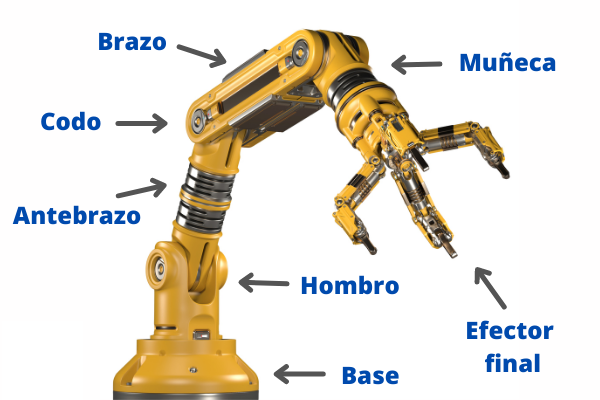
\includegraphics[width=9cm]{figs/brazo_industrial}
  \end{center}
  \caption{\centering Partes de un brazo robótico industrial.}
  \label{fig:brazo_industrials}
\end{figure}

\section{Evolución e historia de la robótica industrial}
\label{sec:segundaseccion}

La robótica industrial aparece por primera vez a mediados del siglo XX en Europa a manos del británico Bill Taylor, estudiante que sobre 1937 creó el robot Gargantua, un robot en forma de grua cuya principal función era la colocación de objetos, dando lugar al primer modelo de pick \& place \footnote{Marketing. (2021, February 2). Historia y Evolución de la Robótica Industrial. EDS Robotics. \url{https://www.edsrobotics.com/blog/evolucion-robotica-industrial/}}. 

Por otro lado, George Devol fue el encargado de crear la primera empresa de robótica de la historia llamada \textit{Unimation} y en el año 1954 se crea el que se considera el primer robot industrial. Este robot consistía en un brazo hidráulico cuya finalidad era elevar cargas pesadas para facilitar su transporte, y en los años siguientes se fueron sacando versiones más avanzadas de este modelo. Además, esta empresa participó en el desarrollo del primer robot de transferencia programable en 1961 \footnote{Robotnik, P. (2021, November 2). Historia \& Origen de los Robots y de la Robótica. Robotnik. \url{https://robotnik.eu/es/historia-de-los-robots-y-la-robotica/}}. \\


\begin{figure}[ht!]
	\centering
	\begin{minipage}{0.44\linewidth}
		\centering
		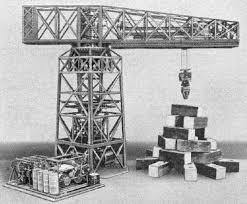
\includegraphics[width=\linewidth]{figs/gargantua.jpg}
		\caption*{\centering Gargantua.}
	\end{minipage}
	\begin{minipage}{0.52\linewidth}
		\centering
		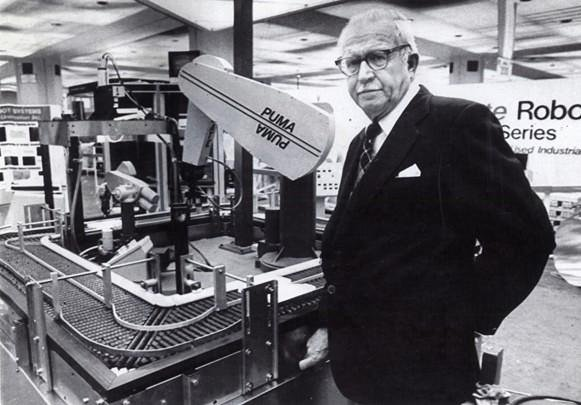
\includegraphics[width=\linewidth]{figs/George_Devol}
		\caption*{\centering George Devol.} 
	\end{minipage}
	\caption{Primeros robots industriales.}
	\label{fig:ancientrel}
\end{figure}

En los años 60 y 70 ya empezaron a aparecer modelos de brazos robóticos más elaborados y de mayor tamaño con elementos como sensores o cámaras incorporados en ellos. En 1973 la empresa alemana KUKA crea Famulus, el primer robot industrial con motores eléctricos y en 1974 Victor Scheinman desarrolla el robot PUMA (Programmable Universal Machine for Assembly), el cual se convierá en un estándar en la industria \footnote{Sutori. (n.d.). Sutori.com. Retrieved February 24, 2025, from \url{ https://www.sutori.com/es/historia/linea-de-tiempo-evolucion-de-la-robotica-industrial--6w6pytow1tj3grr5scVKU1Ns}}. \\

En los años 80 la robótica industrial alcanzó su máximo desarrollo debido a que la fabricación y venta de esta aumentó un 80\% y, aunque EEUU fue el impulsor de esta industria, también empezó a desarrollarse en Asia y Europa. Destaca el robot Motoman L10 de Yaskawa desarrollado en 1981, el cual introduce el uso de retroalimentación por visión, lo que permite a los robots la identificación de objetos y su entorno o el PUMA 560, primer prototipo de robot quirúrgico. 

A partir de la década de 1990, la robótica industrial experimentó un crecimiento significativo, impulsado por la globalización y la creciente demanda de bienes de consumo. Este período marcó la transición hacia la robótica inteligente, estableciendo estándares internacionales por la (ISO) y utilizando sensores avanzados dando lugar a mejores resultados. 

\begin{figure}[ht!]
	\centering
	\begin{minipage}{0.44\linewidth}
		\centering
		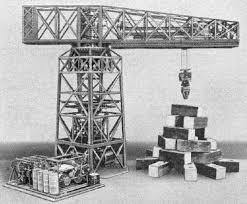
\includegraphics[width=\linewidth]{figs/gargantua.jpg}
		\caption*{\centering Gargantua.}
	\end{minipage}
	\begin{minipage}{0.52\linewidth}
		\centering
		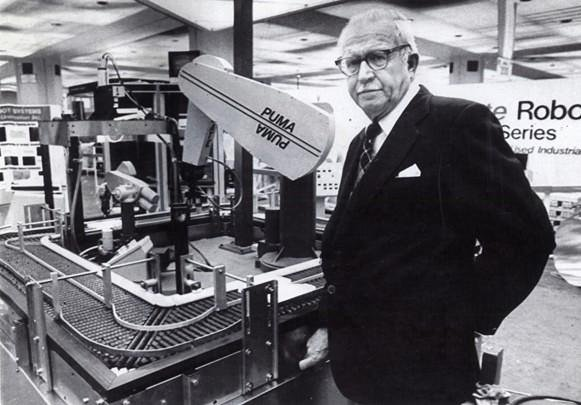
\includegraphics[width=\linewidth]{figs/George_Devol}
		\caption*{\centering George Devol.} 
	\end{minipage}
	\caption{Primeros robots industriales.}
	\label{fig:ancientrel}
\end{figure}

Entrando al siglo XXI se crean los primeros robots colaborativos, conocidos como cobots, concebidos para cooperar de manera directa con las personas. Estos dispositivos se caracterizan por su seguridad, adaptabilidad y facilidad de programación, convirtiéndose en una solución ideal para entornos industriales donde es necesario combinar tareas manuales y automatizadas. 

En los años 2010, la Industria 4.0 emergió como una nueva fase en la manufactura, caracterizada por la digitalización y la interconexión de sistemas de producción. Los robots industriales se convirtieron en componentes clave de las fábricas inteligentes, colaborando estrechamente con humanos y otros sistemas automatizados para optimizar la eficiencia y la flexibilidad en la producción. 




\section{Conceptos fundamentales de la robótica industrial}
\label{sec:terceraseccion}

\section{Beneficios de la automatización con robots industriales}
\label{sec:cuartaseccion}

\section{Motivación del trabajo}
\label{sec:quintaseccion}

En los textos puedes poner palabras en \textit{cursiva}, para aquellas expresiones en sentido \textit{figurado}, palabras como \textit{robota}, que está fuera del diccionario castellano, o bien para resaltar palabras de una colección: \textit{(a)} es la primera letra del abecedario, \textit{(b)} es la segunda, etc.\\



No olvides incluir imágenes y referenciarlas, como la Figura \ref{fig:Robot_intro}.

\subsection{Números}
\label{sec:subseccion}

En lugar de tener secciones interminables, como la Sección \ref{sec:miseccion}, divídelas en subsecciones.

Para hablar de números, mételos en el entorno \textit{math} de \LaTeX, por ejemplo, $1.5Kg$. También puedes usar el símbolo del Euro como aquí: 1.500\euro.

\subsection{Listas}

Cuando describas una colección, usa \texttt{itemize} para ítems o \texttt{enumerate} para enumerados. Por ejemplo:

\begin{itemize}
 \item \textit{Entorno de simulación.} Hemos usado dos entornos de simulación: uno en 3D y otro en 2D.
 \item \textit{Entornos reales.} Dentro del campus, hemos realizado experimentos en Biblioteca y en el edificio de Gestión.
\end{itemize}\

\begin{enumerate}
 \item Primer elemento de la colección.
 \item Segundo elemento de la colección.
\end{enumerate}\

\paragraph{Referencias bibliográficas}
\label{sec:referencias}

Cita, sobre todo en este capítulo, referencias bibliográficas que respalden tu argumento. Para citarlas basta con poner la instrucción \verb|\cite| con el identificador de la cita. Por ejemplo: libros como \cite{vega12e}, artículos como \cite{vega19b}, URLs como \cite{vega19a}, tesis como \cite{vega18b}, congresos como \cite{vega18a}, u otros trabajos fin de grado como \cite{vega08b}.

Las referencias, con todo su contenido, están recogidas en el fichero \texttt{bibliografia.bib}. El contenido de estas referencias está en formato \texttt{BibTex}. Este formato se puede obtener en muchas ocasiones directamente, desde plataformas como \texttt{Google Scholar} u otros repositorios de recursos científicos.

Existen numerosos estilos para reflejar una referencia bibliográfica. El estilo establecido por defecto en este documento es APA, que es uno de los estilos más comunes, pero lo puedes modificar en el archivo \texttt{memoria.tex}; concretamente, cambiando el campo \verb|apalike| a otro en la instrucción \verb|\bibliographystyle{apalike}|. 

\

\

\

Y, para terminar este capítulo, resume brevemente qué vas a contar en los siguientes.
